\documentclass[../main.tex]{subfiles}

\begin{document}

\chapter{Charged Particle Interaction Physics}
The interaction physics that describe the slowing down of energetic light ions through collisions with background charged particles in plasmas are described in terms of differential cross sections. A general collision between an incident energetic light ion of species $x$ and a target charged particle of species $t$ resulting in new species $s$ and $r$ is written as
\begin{equation} \label{eqn:general-collision}
    t(x,s)r,
\end{equation}
where particles $s$ and $r$ are termed the scattered and recoiling particles. The general differential cross section that describes the collision in Eq. \eqref{eqn:general-collision} is
\begin{equation} \label{eqn:differential cross section}
    \sigma_{x,t \rightarrow s}(E^{\prime} \rightarrow E; \mucm),
\end{equation}
where the incident ion, $x$, had energy $E^{\prime}$ before its collision with the target species $t$. The resulting species $s$ is scattered through an angle whose center of mass (CM) cosine is $\mucm$ and has resulting energy $E$. The differential cross section in Eq. \eqref{eqn:differential cross section} is a microscopic differential cross section and has units of $cm^{2}$, and is related to the macroscopic differential cross section as
\begin{equation}
    \Sigma_{x,t \rightarrow s}(E^{\prime} \rightarrow E; \mucm) = \mathcal{N} \sigma_{x,t \rightarrow s}(E^{\prime} \rightarrow E; \mucm),
\end{equation}
where $\mathcal{N}$ is the number density of the target species in $cm^{-3}$.

Collisions where the resulting species is identical to the incident species, $s = x$, are termed elastic scattering collisions; and collisions where the resulting species differs from the incident species, $s \neq x$, are termed nuclear-reaction collisions. These nuclear-reaction collisions result in the destruction of the incident ions and are therefore considered absorption collisions for the incident ion. Furthermore, ion collisions can either be described as light or heavy depending on whether the incident ion is lighter or heavier than the target particle respectively. 

As energetic ions slow down they experience four types of collisions with the background charged particles present in the plasma:
\begin{enumerate}
    \item elastic-Coulomb collisions with thermal electrons;
    \item elastic-Coulomb collisions with thermal ions;
    \item nuclear-elastic scattering (NES) collisions with thermal ions; or
    \item nuclear-reaction collisions with thermal ions.
\end{enumerate}
Because the ion-ion elastic scattering collisions consist of two parts (Coulomb and NES), a quantum mechanical interference differential cross section appears that describes the mutual interference between the two types of elastic scattering collisions \cite{Devaney-1971}. Therefore, the total elastic scattering differential cross section is written as
\begin{equation}
    \sigma_{x,t \rightarrow x} = \sigma_{x,t \rightarrow x}^C + \sigma_{x,t \rightarrow x}^N + \sigma_{x,t \rightarrow x}^I,
\end{equation}
where the superscripts $C$, $N$, and $I$ represent the Coulomb, NES, and interference components of the total ion-ion elastic scattering differential cross section. The differential cross sections that describe Coulomb collisions have an analytical form; while the differential cross sections that describe the NES, interference, and nuclear reactions collisions are tabulated in data sets. The remainder of this section presents the analytical form of the Coulomb differential cross section, and the forms of the tabulated differential cross sections describing the NES, interference, and nuclear-reaction collisions.

% ------------------------------------------------
% COULOMB DIFFERENTIAL CROSS SECTIONS
% ------------------------------------------------
\section{Coulomb Differential Cross Sections}
The Coulomb differential cross section describes the collisions that charged particles experience in a medium as a result of interactions with the charges of the background charged particles present in the plasma. The unscreened and screened Coulomb differential cross sections are found by solving the Schrodinger equation, that is solutions to,
\begin{equation} \label{eqn:Schrodinger}
    \left[-\dfrac{\hbar^2}{2 m}\nabla^2 + k^2 + V(r)\right] \Psi_k(\vec{r}) = \dfrac{(\hbar \vec{k})^2}{2m} \Psi_k(\vec{r}),
\end{equation}
where $m$ is the reduced mass, $k$ is the wave number of the incident particle, and $V(r)$ is the interaction potential. Solutions to Eq. \eqref{eqn:Schrodinger} have at large distances from center of the potential the asymptotic form 
\begin{equation}  \label{eqn:asymptotic-solution}
    \Psi \approx \text{e}^{i\,k\,z} + \dfrac{f(\theta)}{r}\text{e}^{i\,k\,r}
\end{equation}
where the first describes the term describes the incident particle traveling in the positive direction of the z-axis. The second term in Eq. \eqref{eqn:asymptotic-solution} describes the scattered particles as a spherical wave emitted where $f(\theta)$ is some function of the scattering angle characteristic of the interaction potential. In Eq. \eqref{eqn:asymptotic-solution} $f(\theta)$ is often referred to as the scattering amplitude. The differential cross section corresponding to the solution to Eq. \eqref{eqn:Schrodinger} is then found by taking the ratio of the probability per unit time that the scattered particle pass through a surface element $dS = r^2 d\Omega$ to the current density of the incident wave, that is,
\begin{equation} \label{eqn:formula-distinguishable-particles}
    \sigma(E,\theta) = |f(\theta)|^2.
\end{equation}

Collisions where two identical particles collide requires special consideration. This is due to the identity of the particles making it impossible to say which of the particle is scattered and which is recoiling. The differential cross section that describes the interaction of identical particles is
\begin{equation} \label{eqn:formula-identical-particles}
    \sigma_{i}^{C} = | f(\theta) |^2 + | f(\pi - \theta) |^2 + \dfrac{(-1)^{2s}}{2s+1} \left[ f(\theta) f^{\star}(\pi-\theta) + f^{\star}(\theta) f(\pi-\theta) \right],
\end{equation}
where $s$ is the spin of the particles. The first term describes the forward scattering probability, the second term describes the backward scattering probability. The third term in Eq. \eqref{eqn:formula-identical-particles} is an interference term and characterizes the exchange interaction between the forward and backward directions.

In the remainder of this section the analytical forms of the unscreened and screened forms of the Coulomb differential cross section are derived from the scattering amplitudes for both distinguishable and identical particle collisions. Additionally, two different screening functions are introduced: 1) Moliere screening for cold solid materials, and 2) Debye screening for temperature dependent plasmas.

% ------------------------------------------------
% UNSCREENED COULOMB DIFFERENTIAL CROSS SECTIONS 
% ------------------------------------------------
\subsection{Unscreened Coulomb differential cross sections}
The un-screened interaction potential for two charged particles is described by the standard Coulomb potential,
\begin{equation} \label{eqn:Coulomb_potential}
    V(r) = \dfrac{Z_1 \, Z_2 \, e^2}{r},
\end{equation}
where $Z_1 e$ and $Z_2 e$ are the charges of the incident and target charged particles, and $r$ is the distance between the two charges. Note that the Coulomb potential allows for particles that are infinitely far apart to interact with one another, due to the $1/r$ term in Eq. \eqref{eqn:Coulomb_potential}. Solving Schrodinger's equation with the Coulomb potential yields the following scattering amplitude in Coulomb units,
\begin{equation} \label{eqn:coulomb-scattering-amplitude}
    f(\theta) = \dfrac{\gamma}{2 \, k \, \sin^2 \theta/2} \exp \left[ 2 \, i \, \gamma \, \log \sin \theta/2 \right] \dfrac{\Gamma(1 + i/k)}{\Gamma(1 - i/k)},
\end{equation}
where $\gamma = Z_1 \, Z_2 \, e^2 / \hbar \, v$, $v$ is the incident velocity, and $\hbar \, k = \mu \, v$. There are two possible cases for computing the differential cross section that corresponding to Eq. \eqref{eqn:coulomb-scattering-amplitude}: 1) the incident and target particles are distinguishable, and 2) the incident and target particles are identical. 

\subsubsection{Distinguishable particles}
Substituting Eq. \eqref{eqn:coulomb-scattering-amplitude} into Eq. \eqref{eqn:formula-distinguishable-particles} gives
\begin{equation} \label{eqn:dist_unscreened_coulomb}
    \sigma_{d}^{C} = \left(\dfrac{Z_1 \, Z_2 \, e^2}{2 \, \mu \, v^2}\right)^2 \dfrac{1}{\sin^4 \theta/2}
\end{equation}
where $\mu$ is the reduced mass of the system, and $v$ is the velocity of the incident particle. Eq. \eqref{eqn:dist_unscreened_coulomb} can is written in a more usable form by rewriting $e^2 = \alpha \, \hbar c$ and using the half angle trigonometry identity $2 \sin^2 \theta / 2 = 1 - \cos \theta$ to give
\begin{equation}
    \sigma_{d}^{C} = \left(\dfrac{Z_1 \, Z_2 \, \alpha \, \hbar c}{\mu \, v_1^2}\right)^2 \dfrac{1}{(1 - \mucm)^2}, \quad \text{where} \,\, \mucm = \cos \theta.
\end{equation}
Finally, expanding out the reduced mass $\mu = \dfrac{m_1 m_2}{m_1 + m_2}$, and using $m_1 \, v^2 = 2 \, E$ gives
\begin{equation} \label{eqn:coulomb-dcs}
    \sigma_{d}^{C}(E,\mucm) = \left(\dfrac{Z_1^2 \, Z_2^2 \, \left(\alpha \, \hbar c\right)^2}{ 4 \, E^2 \, \left(\frac{A}{1 + A} \right)^2}\right) \dfrac{1}{(1 - \mucm)^2}.
\end{equation}

Figure \ref{fig:sigma_c} shows a plot of Eq. \eqref{eqn:coulomb-dcs} for deuterons colliding with tritons at an incident energy of $1 \mev$ cutoff at $\mucm = 0.99$. Looking at Figure \ref{fig:sigma_c} the Coulomb differential cross section for distinguishable particles is highly peaked about $\mucm = 1$, meaning that particles will most likely undergo collisions that result in zero angular deflection/energy loss. The Coulomb differential cross section has a singularity as $\mucm \rightarrow 1$ due to the Coulomb interaction potential allowing for particles that are infinitely far apart to nonphysically interact with one another. As a result of the singularity Eq. \eqref{eqn:coulomb-dcs} cannot be integrated over the entire range of $\mucm$, and instead must be cutoff. 
\begin{figure}[!htb]
    \centering
    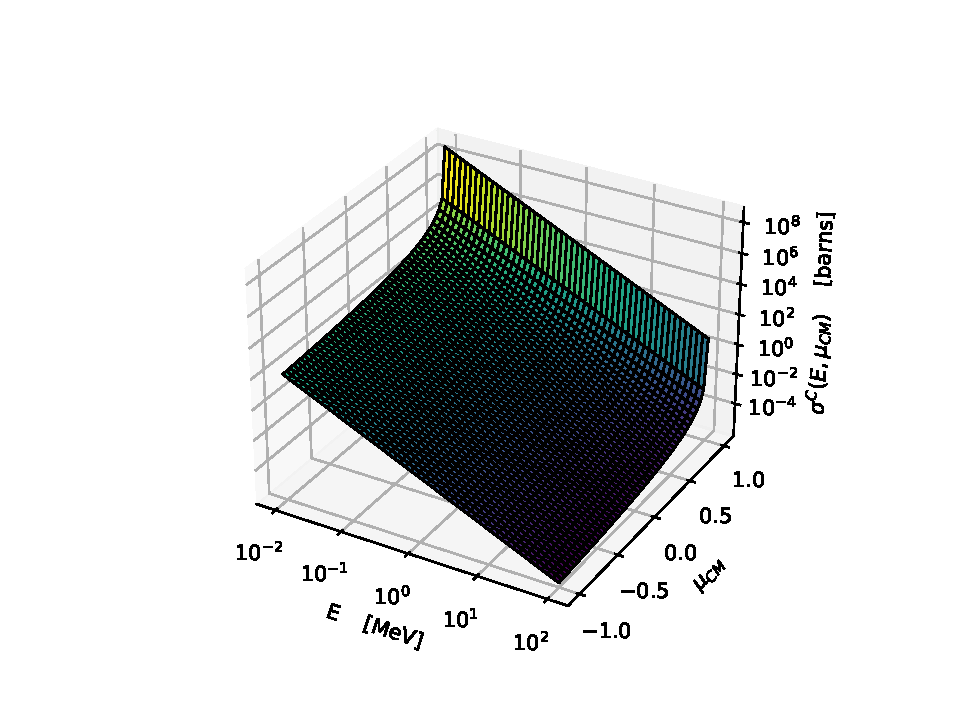
\includegraphics[]{../figures/interaction_physics/sigma-C.pdf}
    \caption{Distinguishable Coulomb differential cross section for energetic deuterons colliding with background tritons cutoff at $\mucm = 0.99$}
    \label{fig:sigma_c}
\end{figure}

The total scattering cross section associated with Eq. \eqref{eqn:coulomb-dcs} is found by integrating over $\mucm$ from $-1$ to some cutoff angle, $\mu_{cut}$ resulting in the following total scattering cross section
\begin{equation} \label{eqn:unscreened-total-xs}
    \sigma^C_d(E) = \left(\dfrac{Z_1^2 \, Z_2^2 \, \left(\alpha \, \hbar c\right)^2}{ 4 \, E^2 \, \left(\frac{A}{1 + A} \right)^2}\right) \dfrac{\mu_{cut}}{1-\mu_{cut}}, \quad \text{where} \,\, -1 < \mu_{cut} < 1.
\end{equation}
Figure \ref{fig:sigma_c_total} shows Eq. \eqref{eqn:unscreened-total-xs} for several different collisions and with a cutoff cosine of $\mu_{cut} = 0.999$. From Figure \ref{fig:sigma_c_total} as the energy of the incident particle increases the magnitude of the total cross section decreases, this can also be seen in Figure \ref{fig:sigma_c}. Additionally, as the mass of the incident particle increases so does the magnitude of the total cross section. Conversely, as the mass of the target particle increases, the magnitude of the of the total cross section decreases. Lastly, for nominal ICF energies, $<10$ MeV, the magnitude of Eq. \eqref{eqn:unscreened-total-xs} is large ($>1$ barn) meaning that for typical ICF densities the mean free path is very small and highly peaked about zero angular deflection.
\begin{figure}[!htb]
    \centering
    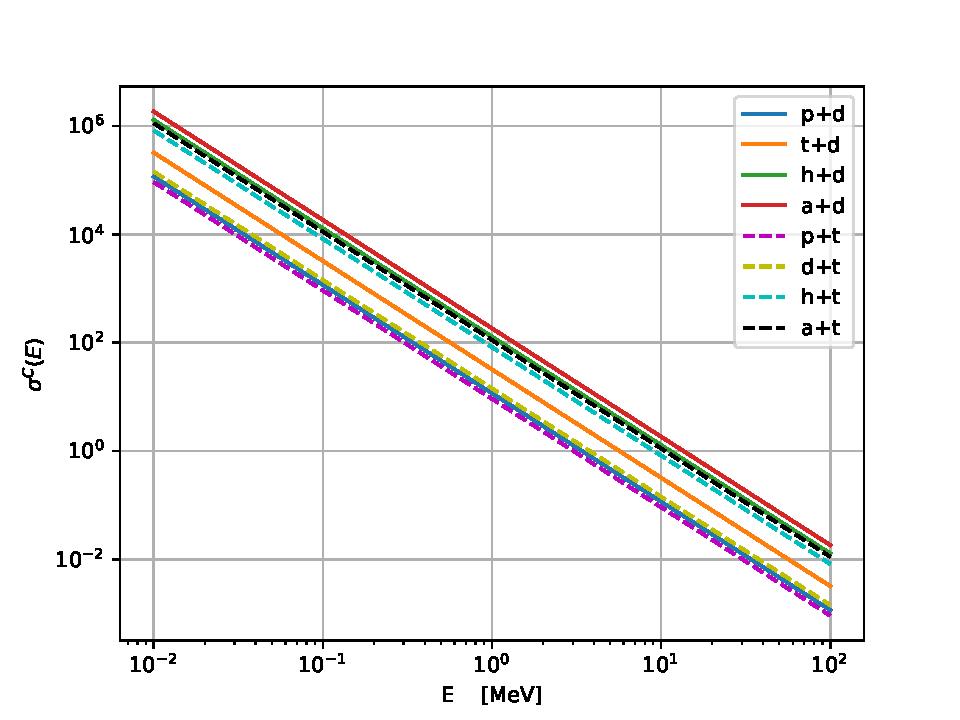
\includegraphics[scale=0.75]{../figures/interaction_physics/total-sigma-C.pdf}
    \caption{Total distinguishable Coulomb differential cross section for several collisions cutoff at $\mucm = 0.999$}
    \label{fig:sigma_c_total}
\end{figure}

\subsubsection{Identical particles}
Substituting Eq. \eqref{eqn:coulomb-scattering-amplitude} into Eq. \eqref{eqn:formula-identical-particles} gives the un-screened Coulomb differential cross section for identical particles, that is,
\begin{multline} \label{eqn:coulomb-unscreened-identical}
   \sigma_{i}^{C} = \dfrac{\gamma^2}{k^2} \left[ \dfrac{1}{(1 - \mucm)^2} + \dfrac{1}{(1 + \mucm)^2} \right. \\ \left. + \dfrac{(-1)^{2s}}{2s+1} \dfrac{2}{(1 - \mucm)(1 + \mucm)} \cos \left( \gamma \, \log \, \dfrac{1 - \mucm}{1 + \mucm} \right) \right].
\end{multline}
Figure \ref{fig:coulomb-identical} shows $\sigma_{C,i}$ for a variety of incident particle energies and cosine of CM scattering angles. From Figure \ref{fig:coulomb-identical} the identical particle differential cross section is highly peaked about $\mucm = -1, 1$ due to the Coulomb interaction potential. 
\begin{figure}[!htb]
    \centering
    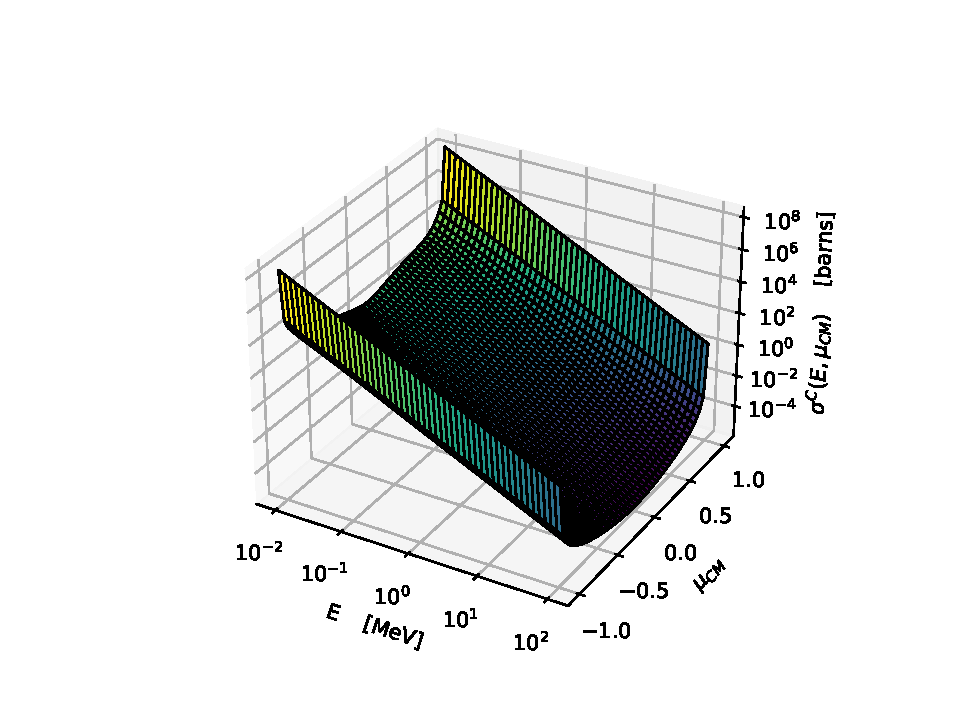
\includegraphics[]{../figures/interaction_physics/sigma-Ci.pdf}
    \caption{The identical particle Coulomb differential cross section for deuterons colliding with background deuterons for $\mucm = [-0.99,0.99]$}
    \label{fig:coulomb-identical}
\end{figure}

Eq. \eqref{eqn:coulomb-unscreened-identical} can be greatly simplified when $\gamma \ll 1$ meaning that the velocity of the incident particle is so large that $\hbar v \gg Z_1 Z_2 e^2$. In this case the cosine in the third term can be replaced by unity and Eq. \eqref{eqn:coulomb-unscreened-identical} becomes
\begin{equation} \label{eqn:coulomb-unscreened-identical-simplified}
   \sigma_{i}^{C} \approx \dfrac{2 \, \gamma^2}{k^2 (1 - \mucm^2)} \left[\dfrac{1+ \mucm^2}{1-\mucm^2} + \dfrac{(-1)^{2s}}{2s+1}\right], \quad \text{when} \,\, \gamma \ll 1.
\end{equation}
For the opposite case, $\hbar v \ll Z_1 Z_2 e^2$, the cosine term in Eq. \eqref{eqn:coulomb-unscreened-identical} is a rapidly oscillating function, and the resulting cross section differs significantly from the Rutherford value given by Eq. \eqref{eqn:coulomb-unscreened-identical-simplified}. Figure \ref{fig:coulomb-identical-2d} shows the oscillations in the differential cross section due to the cosine term at various incident particle energies. In Figure \ref{fig:coulomb-identical-2d} it is clear that at low energies ($E < 10$ keV) these oscillations are significant; however, at higher energies these oscillations atr not significant and the Eq. \eqref{eqn:coulomb-unscreened-identical} rapidly approaches Eq. \eqref{eqn:coulomb-unscreened-identical-simplified}.

\begin{figure}[!htb]
    \centering
    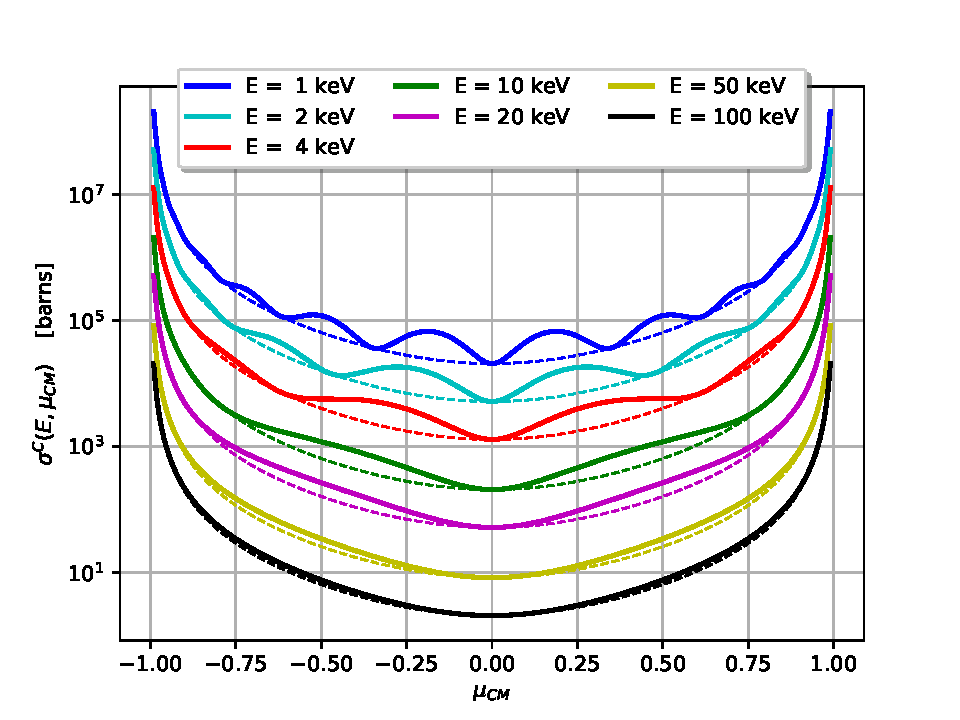
\includegraphics[]{../figures/interaction_physics/sigma-Ci-2d.pdf}
    \caption{Comparison between the full (solid lines) and approximate (dashed lines) identical particle Coulomb differential cross sections at various energies for tritons colliding with background tritons for $\mucm = [-0.99,0.99]$.}
    \label{fig:coulomb-identical-2d}
\end{figure}

% ------------------------------------------------
% SCREENED COULOMB DIFFERENTIAL CROSS SECTIONS 
% ------------------------------------------------
\subsection{Screened coulomb differential cross sections}
To overcome the difficulties of the Coulomb interaction potential, namely the fact that it allows for particle infinitely far apart to interact with one another, Wentzel and Yukawa independently introduced the screened Coulomb potential,
\begin{equation} \label{eqn:wentzel-interaction-potential}
    V_s(r) = \dfrac{Z_1 \, Z_2 \, e^2}{r} \exp \left(-\frac{r}{R}\right),
\end{equation}
where $R$ is the characteristic screening length of the system. In Eq. \eqref{eqn:wentzel-interaction-potential} exponential term decreases more rapidly than the $1/r$ term thereby making the probability that particles will interact at distances greater than $R$ exponentially decreases with increasing interaction length $r$. This leads to an interaction potential that is finite as $r \rightarrow \infty$ while still have the same general behavior as the original Coulomb interaction potential.

The Schrodinger equation with the screened Coulomb interaction potential cannot be solved exactly and therefore its solution is approximated with the Born approximation. The Born approximation consists of approximating the the scattered wave function by a plane wave, and gives the following formula for the scattering amplitude
\begin{equation} \label{eqn:first-born-approximation}
    f(\theta) \approx - \dfrac{2 \, m}{\hbar^2} \int\limits_0^{\infty} U(r) \, \dfrac{\sin qr}{q} \, r \, dr
\end{equation}
where $q = 2 \, k \, \sin \theta / 2$. Substituting the screened interaction potential into Eq. \eqref{eqn:first-born-approximation} and yields
\begin{equation} \label{eqn:wentzel-scattering-amplitude}
    f_s(\theta) = \dfrac{Z_1 \, Z_2 \, e^2 \, m}{2 \, k^2 \, \hbar^2} \dfrac{1}{(2kR)^{-2} + \sin^2 \theta/2} = \dfrac{\gamma}{2 \, k} \left[\dfrac{1}{(2kR)^{-2} + \sin^2 \theta/2}\right].
\end{equation}
In Eq. \eqref{eqn:wentzel-scattering-amplitude} the term $(2kR)^{-2}$ is often referred to as the screening parameter and is denoted by $A_s$. Note that as $A_s \rightarrow 0$ Eq. \eqref{eqn:wentzel-scattering-amplitude} approaches the unscreened Coulomb potential scattering amplitude, Eq. \eqref{eqn:Coulomb_potential}, without the exponential and gamma function terms. In fact it has been shown that the Born approximation is not a valid approximation of the scattering amplitude when a screened interaction potential is used for nucleon-nucleon interactions unless the incident particles energy is at relativistic speeds. Nonetheless, the differential cross sections for distinguishable and identical particles are derived using Eq. \eqref{eqn:wentzel-scattering-amplitude} as they result in differential cross sections that are at least finite at $\mucm = 1$ and resemble the Coulomb differential cross sections previously derived.

Using Eqs. \eqref{eqn:formula-distinguishable-particles} and \eqref{eqn:formula-identical-particles} the screened Coulomb differential cross section for distinguishable and identical particles are
\begin{equation} \label{eqn:screened-coulomb-d}
    \sigma_{d}(E,\mucm) = \dfrac{\gamma^2}{k^2} \dfrac{1}{\left[A_s + 1 - \mucm\right]^2},
\end{equation}
and
\begin{multline} \label{eqn:screened-coulomb-i}
    \sigma_{i}(E,\mucm) = \dfrac{\gamma^2}{k^2} \left[ \dfrac{1}{\left(A_s + 1 - \mucm\right)^2} + \dfrac{1}{\left(A_s + 1 + \mucm\right)^2} \right. \\ \left. + \dfrac{(-1)^{2s}}{2s+1} \dfrac{2}{\left(A_s + 1 - \mucm\right)\left(A_s + 1 + \mucm\right) }\right].
\end{multline}
In Eq. \eqref{eqn:screened-coulomb-d} as $A_s \rightarrow 0$ it becomes the unscreened Coulomb differential cross sections (Eq. \eqref{eqn:coulomb-dcs}). However, in the identical particle case as $A_s \rightarrow 0$ instead of approaching the unscreened identical particle differential cross Eq. \eqref{eqn:screened-coulomb-i} becomes the approximate unscreened identical particle differential cross section (Eq. \eqref{eqn:coulomb-unscreened-identical-simplified}). This discrepancy is due to the validity of the Born approximation, which is only valid if the incident particle has high energy. However, Eqs. \eqref{eqn:screened-coulomb-d} and \eqref{eqn:screened-coulomb-i} are considered ``good enough'' approximations to the true differential cross section and are used throughout the remainder of this dissertation. 

% ------------------------------------------------
% SCREENING FUNCTIONS 
% ------------------------------------------------
\subsection{Screening Functions}
In this section the various screening functions for the Coulomb differential cross section that are available in LANDO are described. Additionally, we describe how to use a custom screening function. There are four screening functions provided in LANDO: none, constant, Moliere, and Debye. The following subsection discuss each of these functions.


\subsubsection{Moliere screening}
Moliere screening describes the screening of the nuclear charge of a nucleus due to the atomic electrons in the atom. The formula for Moliere screening is
\begin{equation}
    A_s^M(E) = \left( \dfrac{\hbar c}{2 \, pc \, a_I}\right)^2 \left[ 1.13 + 3.76  \, \left( \dfrac{\alpha \, z \, Z}{\beta}\right)\right]
\end{equation}
where $\hbar c$ is the reduced Planck constant; $\alpha$ is the fine structure constant; $pc$ is the momentum of the incoming particle; $z$ is the charge of the incoming particle; $Z$ is the charge of the target particle; $a_I$ is the universal screening length. The universal screening length is given by
\begin{equation}
    a_I = 
    \begin{cases}
        \quad \dfrac{C_{TF} \, a_0}{Z^{1/3}}, \quad\quad &z = 1 \\\\
        \dfrac{C_{TF} \, a_0}{z^{0.23} + Z^{0.23}}, \quad &z \geq 2
    \end{cases}, \quad
    C_{TF} = \dfrac{1}{2} \left( \dfrac{3 \, \pi}{4}\right)^{2/3}.
\end{equation}

Moliere screening can be used in LANDO by using the following screening function

\subsubsection{Debye screening}
Debye screening is a measure of a charge carrier's net electrostatic effect in a solution and how far its electrostatic effect persists. The Debye length is computed as
\begin{equation}
    \lambda_D = \left[ \epsilon_0 \sum_{j=0}^N \dfrac{k_B T_j}{z_j^2 \, n_j} \right]^{-1/2}
\end{equation}
where the index $j$ indicates the background species.

Debye screening can be used in LANDO by using the following screening function

\begin{figure}[!htb]
    \centering
    \begin{minipage}{.5\textwidth}
      \centering
      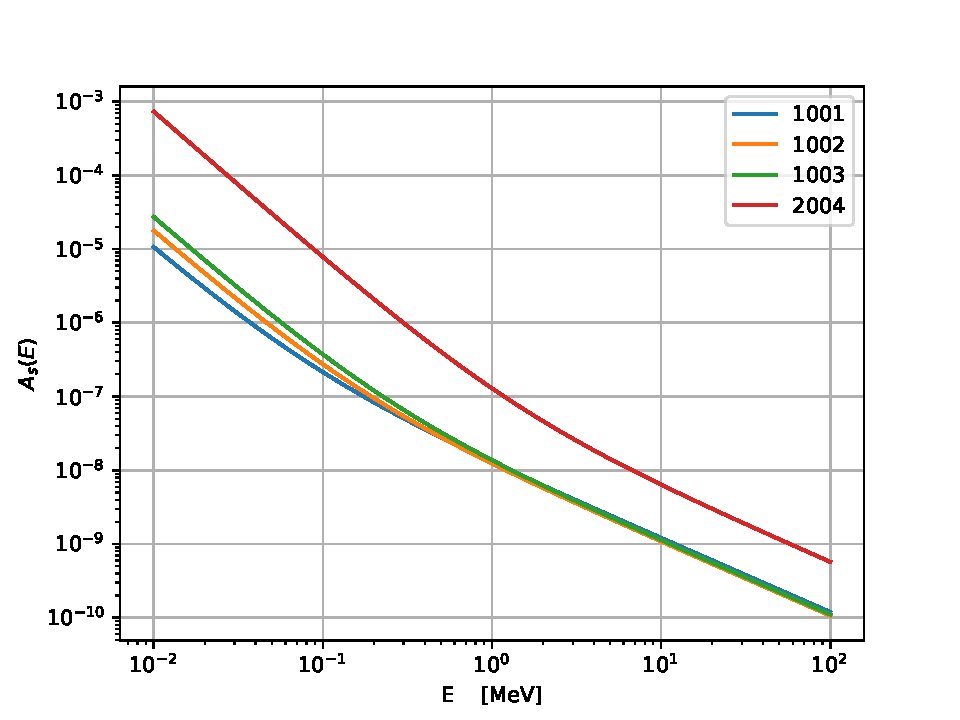
\includegraphics[width=\linewidth]{../figures/interaction_physics/moliere-screening.pdf}
      \captionof{figure}{A figure}
      \label{fig:test1}
    \end{minipage}%
    \begin{minipage}{.5\textwidth}
      \centering
      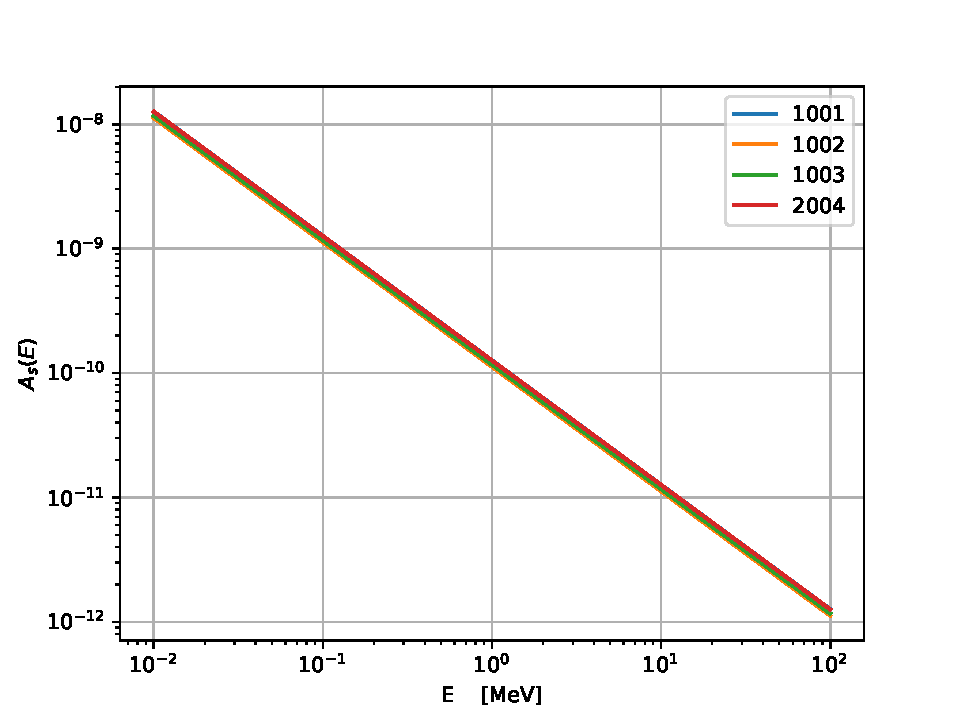
\includegraphics[width=\linewidth]{../figures/interaction_physics/debye-screening.pdf}
      \captionof{figure}{Another figure}
      \label{fig:test2}
    \end{minipage}
\end{figure}

% ------------------------------------------------
% NES DIFFERENTIAL CROSS SECTIONS 
% ------------------------------------------------
\subsection{Nuclear Elastic Scattering}
Nuclear elastic scattering collisions are short-range collisions that can result in large angular deflections. The NES differential cross sections are expressed in terms of Legendre moments,
\begin{equation} \label{eqn:nes_differential cross section}
    \sigma_{x,t \rightarrow x}^N(E^{\prime} \rightarrow E; \mucm) = \sum_{l=0}^L \dfrac{2l+1}{2} b_l(E^{\prime}) P_l(\mucm),
\end{equation}
where $P_l(\mucm)$ are the Legendre polynomials of order $l$, and $b_l(E)$ are the tabulated Legendre expansion coefficients \cite{Brown-2018}.

Figure \ref{fig:nesTotal} shows the total NES cross sections for DD, DT, DH, and DA collisions. In Figure \ref{fig:nesTotal}, as the energy of the incident particle increases so does the total NES cross sections. These NES cross sections are much smaller in magnitude than the corresponding Coulomb cross sections at low incident energies, $\sim 10^4$ barns at $0.1 \mev$. However, at high energies, $(> 1 \mev)$, the NES and Coulomb cross sections become comparable in magnitude with the Coulomb cross section varying between $10^2$ and $10^0$ barns between incident particle energies of $1 \mev$ and $10 \mev$. In general then, the slowing down of low energy particles $(< 1 \mev)$ is dominated by Coulomb collisions whereas the slowing down of energetic particles $(> 1 \mev)$ is caused by a combination of both Coulomb and NES collisions.

\begin{figure}[!htb]
    \centering
    \includegraphics[scale=0.75]{../figures/chapter-4/sigmaNES_total.pdf}
    \caption{Total nuclear elastic scattering cross sections}
    \label{fig:nesTotal}
\end{figure}

In Figure \ref{fig:nesDCS} the NES differential cross section for the DT collision is shown at various incident particle energies. From Figure \ref{fig:nesDCS}, at low incident particle energies the scattering is approximately isotropic; however, at high energies there is a significant probably of scattering in backward directions. Scattering in backward directions causes the particles to lose a significant amounts of energy in single collisions. Therefore at high energies there is a significant probability that a particle will lose a considerable amount of energy causing it to slow down quicker than if only Coulomb collisions are taken into account. Nakao et al. \cite{Nakao-1990} examined the effects of NES on the slowing down of energetic light ions in ICF plasmas and found that they contributed significantly for high energy, $(> 10 \mev)$, protons slowing down in a DT plasma.

\begin{figure}[!htb]
    \centering
    \includegraphics[scale=0.75]{../figures/chapter-4/sigmaNES_dcs.pdf}
    \caption{Nuclear elastic scattering differential cross section for DT}
    \label{fig:nesDCS}
\end{figure}

% ------------------------------------------------
% INTERFERENCE DIFFERENTIAL CROSS SECTIONS 
% ------------------------------------------------
\section{Interference Differential Cross Sections}
In Figure \ref{fig:sig_i}, the interference differential cross section for energetic deuterons colliding with tritons is shown for various incident energies. Looking at Figure \ref{fig:sig_i}, as $\mucm \rightarrow 1$ the interference differential cross section oscillates between positive and negative values of increasing magnitude. Negative differential cross sections have no physical meaning, and therefore the interference differential cross section must be combined some other differential cross section such that the resulting differential cross section is always positive.

\begin{figure}[!htb]
    \centering
    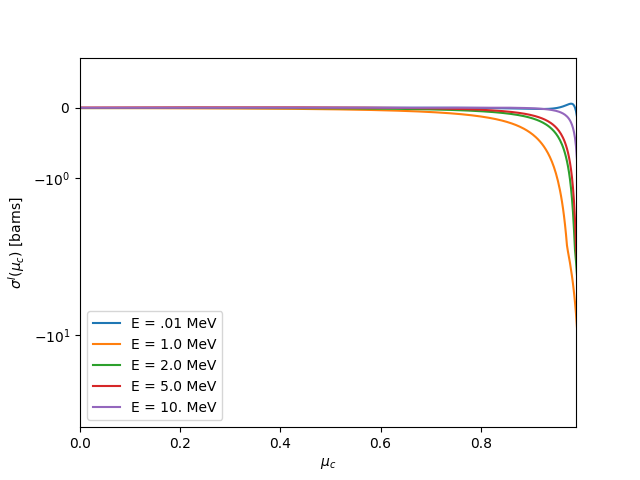
\includegraphics[scale=0.75]{../figures/proposed_work/sig_i_dt.png}
    \caption{Interference scattering differential cross section for deuterons colliding with tritons at 1.0 MeV}
    \label{fig:sig_i}
\end{figure}

% ------------------------------------------------
% NUCLEAR REACTION DIFFERENTIAL CROSS SECTIONS 
% ------------------------------------------------
\section{Thermonuclear Reactions}
Thermonuclear (TN) reactions are collisions that cause the identities of the emitted particles to differ from the incident and target particles. There are 4 main nuclear reactions of interest in ICF applications which are typically reffered to as the big 4, they are:
\begin{multicols}{2}
\begin{itemize}
    \item $\ce{^{2}_{1}H} \, (t, \, n)\, \ce{^{4}_{2}He}$  $(Q = 10.0 \mev)$
    \item $\ce{^{3}_{2}He}\, (d, \, p)\, \ce{^{4}_{2}He}$  $(Q = 10.0 \mev)$
    \item $\ce{^{2}_{1}H} \, (d, \, n)\, \ce{^{3}_{2}He}$  $(Q = 10.0 \mev)$
    \item $\ce{^{2}_{1}H} \, (d, \, p)\, \ce{^{3}_{1}H}$   $(Q = 10.0 \mev)$
\end{itemize}
\end{multicols}
where $Q$ is the Q-value of the reaction. The three reacting isotopes, (d,t,h), produce seven charged particle products plus two neutron products. TN reactions cause the energy spectrum of charged particles and neutrons to vary from thermal background temperatures all the way up to $\sim 30 \mev$. TN reactions are typically divided into primary reactions, and secondary reactions (fusion of a primary product). In addition, tertiary interactions utilizing both processes in sequence can produce particles with the highest energy.  

Figure \ref{fig:tnTotal} shows the total TN reaction cross sections for the major four reactions. In Figure \ref{fig:tnTotal} we see that the TN reaction with the highest probability is the deuterium-tritium reaction with a peak at $0.1 \mev$ of $\sim 4 \barns$. The next largest TN reaction is the deuterium-helion reaction with a peak at $0.4 \mev$ of $\sim 1 \barns$; however, most ICF background plasmas do not contain appreciable amounts of $\ce{^{3}_{2}He}$ and therefore this reaction is considered a secondary reaction because only helions produce from deuterium-deuterium reactions can produce the necessary helions. The two deuterium-deuterium reactions occur with roughly equal probability. It is also worth noting that at high energies ($> 2 \mev$) all the TN reactions occur with equal probability.

\begin{figure}[!htb]
    \centering
    \includegraphics[scale=0.75]{../figures/chapter-4/tnTotal.pdf}
    \caption{Total thermonuclear reaction cross sections}
    \label{fig:tnTotal}
\end{figure}

Figure \ref{fig:tnDiffernetialCrossSections} shows the angular dependence of the TN differential cross sections at various energies for the DD and DT reactions. From Figure \ref{fig:tnDiffernetialCrossSections}, the neutron emitted in the DT reaction is emitted fairly isotopically at low energies. However, as the energy of the incident deuteron increases, the outgoing neutron is increasingly more likely to emitted in forward directions. Similarly, in the DD reaction there is slight bias in the forward direction at low incident particle energies and increases with increasing incident particle energy. In general, it can be concluded in TN reactions that the light particle tends to scatter in forward directions while the heavy particle will scatter in backward directions.

\begin{figure}[!htb]
  \centering
  \begin{subfigure}{.45\textwidth}
    \centering
    \includegraphics[scale=0.45]{../figures/chapter-4/ddDCS.pdf}
    \caption{$d + d \rightarrow p + h$}
    \label{fig:ddDCS}
  \end{subfigure}%
  \begin{subfigure}{.45\textwidth}
    \centering
    \includegraphics[scale=0.45]{../figures/chapter-4/dtDCS.pdf}
    \caption{$d + t \rightarrow n + a$}
    \label{fig:dtDCS}
  \end{subfigure}
  \caption{Thermonuclear reaction differential cross sections}
  \label{fig:tnDiffernetialCrossSections}
\end{figure}

\end{document}
